\chapter{Résultats et perspective future}

\section{Résultats}

La figure \ref{fig:rmf_800} est un example de résultat obtenue à partir d'un bruit \textit{RIDGED MULTI FRACTAL}. 

\begin{figure}
    \centering
    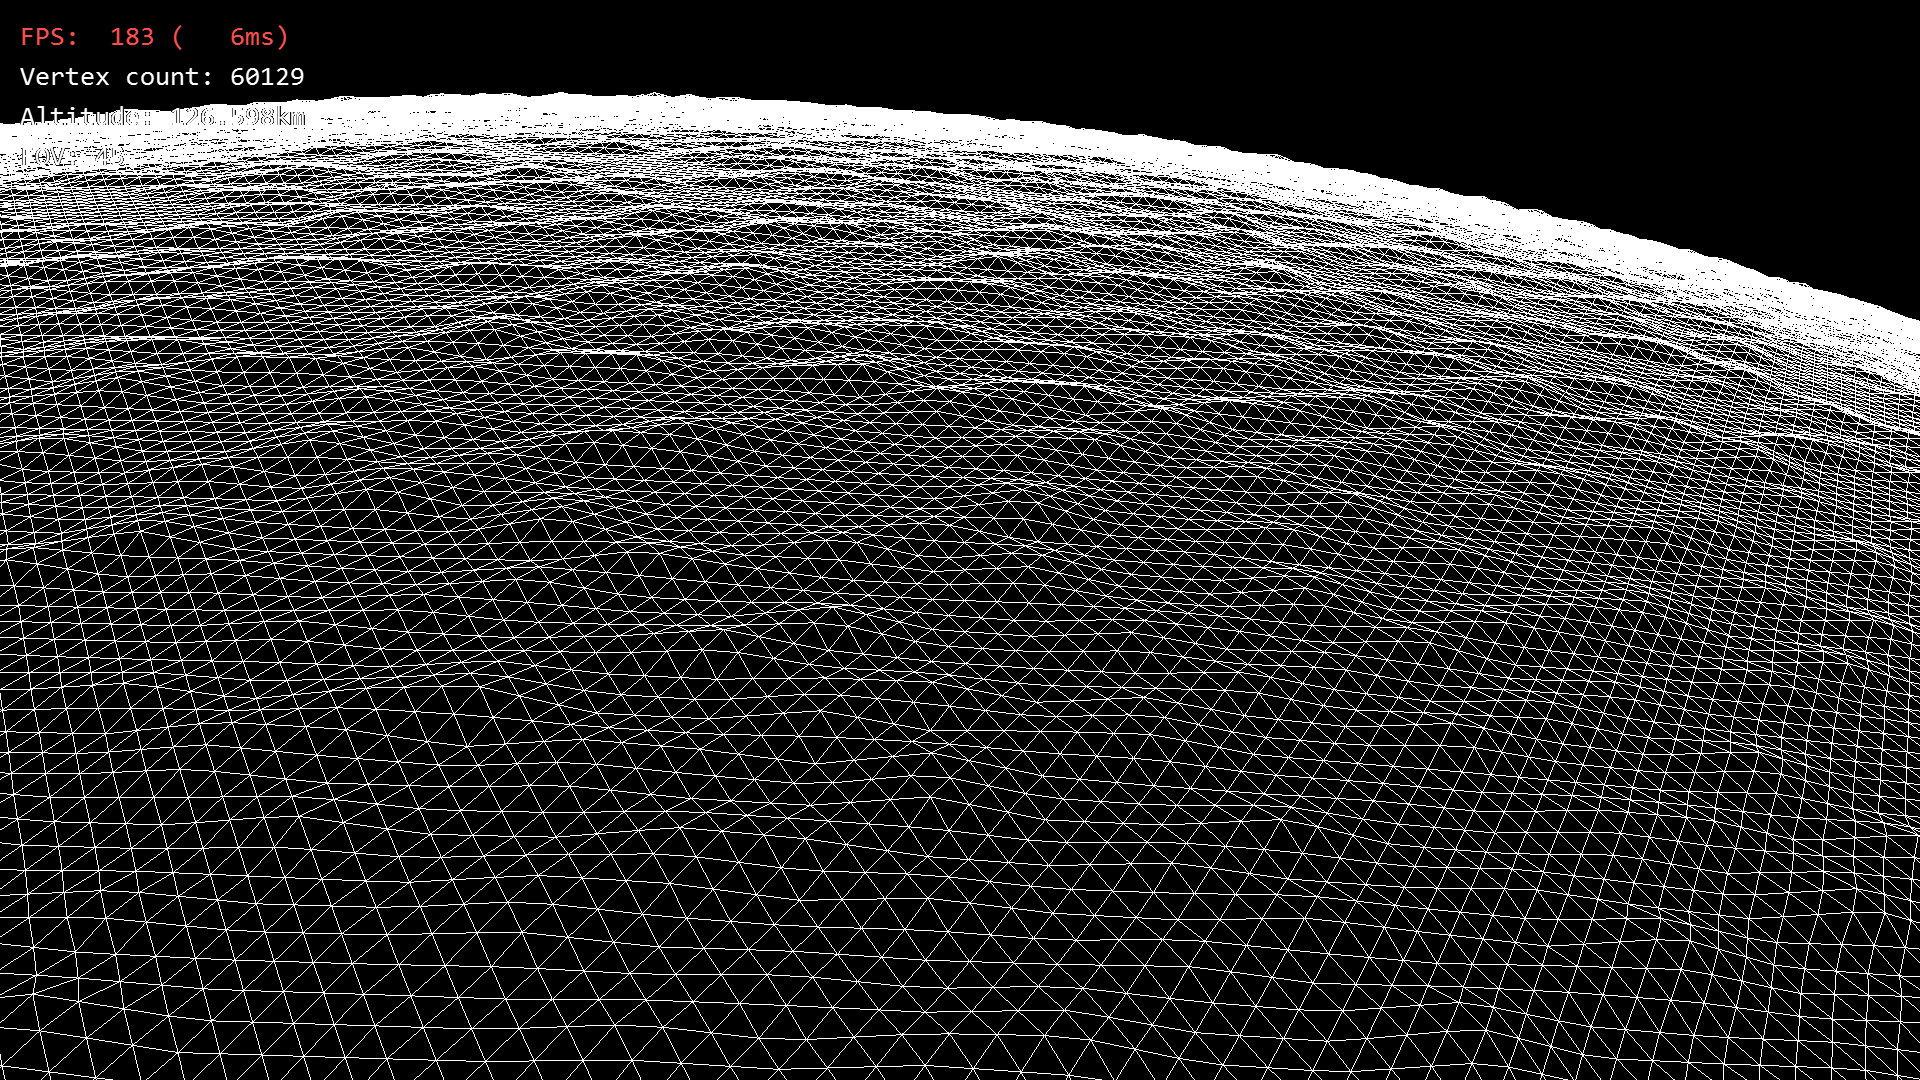
\includegraphics[width=10cm]{img/RMFV_w800_h800_wire_0.png}
    \caption{./ProceduralPlanet RIDGED-MULTI-FRACTAL --width=800 --height=800}
    \label{fig:rmf_800}
\end{figure}

Ce bruit est un bruit basé sur simplex, la figure \ref{fig:rmf} est une représentation sur deux dimension de ce bruit. 
Le bruit de la figure \ref{fig:rmf} et le bruit appliqué sur la planète ne sont pas identique, la figure \ref{fig:rmf} n'est qu'une représentation.

\begin{figure}
    \centering
    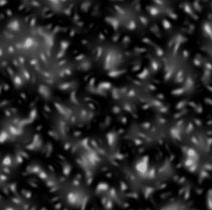
\includegraphics[width=10cm]{img/RMF.jpg}
    \caption{RIDGED MULTI FRACTAL, source \url{https://github.com/simongeilfus/SimplexNoise}, dernier accès Mars 2018}
    \label{fig:rmf}
\end{figure}

\subsection{Limitation}

Pour avoir une planète correcte, on peut voir qu'il est nécessaire de créer une carte de hauteur de faible résolution. Cependant cela fait apparaître de la pixelisation sur la planète. Cela est du au calcul de la lumière faite dans le \textit{shader} qui ce base sur les hauteurs. La figure \ref{fig:px_ombre} montre se phénomène. \\

%Parler du clipping des textures.


\begin{figure}
    \centering
    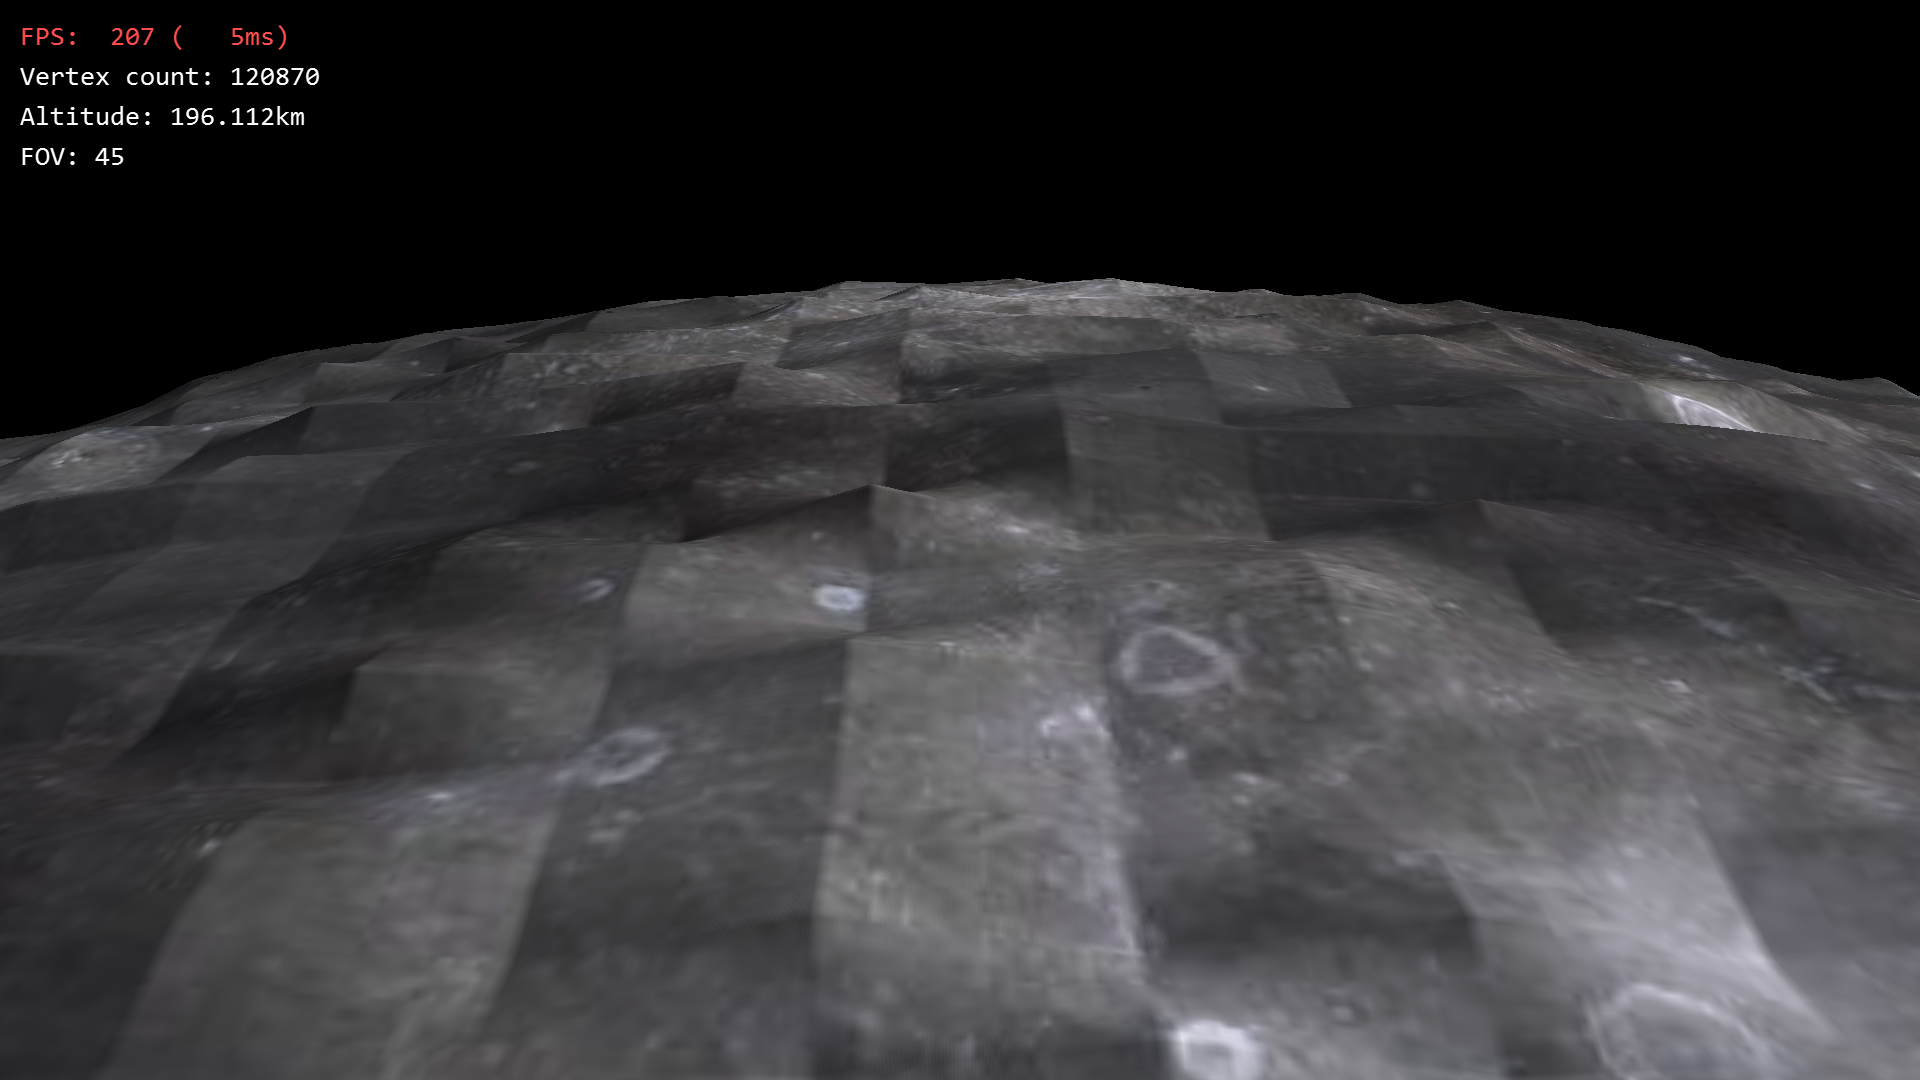
\includegraphics[width=10cm]{img/SIMPLEX_w200_h200_0.png}
    \caption{Pixelisation des ombres}
    \label{fig:px_ombre}
\end{figure}


\section{Perspective future}

Des améliorations peuvent encore être apportées dans le futur.
Tous d'abord il serait très vite nécessaire de changer le système de calcul de la lumière. 
%Les détails d'implémentation de celui utilisé actuellement sont expliqué dans la partie \ref{sec:phong}

Le remplacer par un autre qui ne créer pas les problèmes de pixelisation des ombres que l'on peut voir sur l'image \ref{fig:px_ombre}.\\

Il peut être par exemple remplacé par un calcul des couleurs en fonction de l'altitude. C'est à dire affecter une couleur différente suivant la hauteur du sommet. Cela permettrait de facilement visualiser les hauteurs.\\

Il peut être envisagé d'utiliser \textit{OpenMP} pour accélérer la génération de la texture. Cette amélioration n'est pas essentielle au vue de la résolution des textures qui sont générées mais cela peut avoir un impact non négligeable sur des textures plus grande.

\textit{OpenMP} est une bibliothèque permettant de facilité le calcule d'une tâche sur plusieurs processeurs.

%Plus de bruit !!!
%Corriger les probalèmes avec la lumière
%Visualiser la hauteur avec une couleur
%OpenMP